%\documentclass{article}
%\usepackage[utf8]{inputenc}

%\title{Thesis Anabel}
%\author{anabel_dlw }
%\date{June 2017}

%\begin{document}

%\maketitle

%\section{Introduction}

%\end{document}


\documentclass[
		twoside,openright,titlepage,numbers=noenddot,headinclude,%1headlines,
	 	cleardoublepage=empty,
		dottedtoc, % Make page numbers in the table of contents flushed right with dots leading to them
		BCOR=5mm,paper=a4,fontsize=11pt, % Binding correction, paper type and font size
		ngerman,american, % Languages, change this to your language(s)
		]{scrreprt} 
                
% Includes the file which contains all the document configurations and packages - make sure to edit this file
\PassOptionsToPackage{utf8}{inputenc} % Set the encoding of your files. UTF-8 is the only sensible encoding nowadays. If you can't read äöüßáéçèê∂åëæƒÏ€ then change the encoding setting in your editor, not the line below. If your editor does not support utf8 use another editor!
\usepackage{inputenc}

%----------------------------------------------------------------------------------------
%	DOCUMENT VARIABLES
%	Fill in the lines below to enter your information into the thesis template
%	Each of the commands can be cited anywhere in the thesis
%----------------------------------------------------------------------------------------

% Remove drafting to get rid of the '[ Date - classicthesis version 4.0 ]' text at the bottom of every page
\PassOptionsToPackage{eulerchapternumbers,listings,drafting, pdfspacing, subfig,beramono,eulermath,parts}{classicthesis}
% Available options: drafting parts nochapters linedheaders eulerchapternumbers beramono eulermath pdfspacing minionprospacing tocaligned dottedtoc manychapters listings floatperchapter subfig

\newcommand{\myTitle}{SDN support within Neutron for container-based deployments \xspace}
\newcommand{\mySubtitle}{Nada\xspace}
\newcommand{\myDegree}{ing\xspace}
\newcommand{\myName}{Anabel Larrea\xspace}
\newcommand{\myProf}{Ph\xspace}
\newcommand{\myOtherProf}{Put name here\xspace}
\newcommand{\mySupervisor}{Dr inż. Krzysztof Wajda\xspace}
\newcommand{\myFaculty}{Networks and services\xspace}
\newcommand{\myDepartment}{Put data here\xspace}
\newcommand{\myUni}{Put data here\xspace}
\newcommand{\myLocation}{Saarbrücken\xspace}
\newcommand{\myTime}{2017\xspace}
\newcommand{\myVersion}{version 4.2\xspace}

%----------------------------------------------------------------------------------------
%	USEFUL COMMANDS
%----------------------------------------------------------------------------------------

\newcommand{\ie}{i.\,e.}
\newcommand{\Ie}{I.\,e.}
\newcommand{\eg}{e.\,g.}
\newcommand{\Eg}{E.\,g.} 

\newcounter{dummy} % Necessary for correct hyperlinks (to index, bib, etc.)
\providecommand{\mLyX}{L\kern-.1667em\lower.25em\hbox{Y}\kern-.125emX\@}
\newlength{\abcd} % for ab..z string length calculation

%----------------------------------------------------------------------------------------
%	PACKAGES
%----------------------------------------------------------------------------------------

\usepackage{lipsum} % Used for inserting dummy 'Lorem ipsum' text into the template

%------------------------------------------------

%\PassOptionsToPackage{ngerman,american}{babel}  % Change this to your language(s)
% Spanish languages need extra options in order to work with this template
%\PassOptionsToPackage{spanish,es-lcroman}{babel}
\usepackage{babel}

%------------------------------------------------			

\usepackage{csquotes}
\PassOptionsToPackage{%
%backend=biber, % Instead of bibtex
backend=bibtex8,bibencoding=ascii,%
language=auto,%
style=numeric-comp,%
%style=authoryear-comp, % Author 1999, 2010
%bibstyle=authoryear,dashed=false, % dashed: substitute rep. author with ---
sorting=nyt, % name, year, title
maxbibnames=10, % default: 3, et al.
%backref=true,%
natbib=true % natbib compatibility mode (\citep and \citet still work)
}{biblatex}
\usepackage{biblatex}
 
 %------------------------------------------------

\PassOptionsToPackage{fleqn}{amsmath} % Math environments and more by the AMS 
 \usepackage{amsmath}
 
 %------------------------------------------------

\PassOptionsToPackage{T1}{fontenc} % T2A for cyrillics
\usepackage{fontenc}

%------------------------------------------------

\usepackage{textcomp} % Fix warning with missing font shapes

%------------------------------------------------

\usepackage{scrhack} % Fix warnings when using KOMA with listings package  

%------------------------------------------------

\usepackage{xspace} % To get the spacing after macros right

%------------------------------------------------

\usepackage{mparhack} % To get marginpar right

%------------------------------------------------

\usepackage{fixltx2e} % Fixes some LaTeX stuff 

%------------------------------------------------

\PassOptionsToPackage{smaller}{acronym} % Include printonlyused in the first bracket to only show acronyms used in the text
\usepackage{acronym} % Nice macros for handling all acronyms in the thesis

%\renewcommand*{\acsfont}[1]{\textssc{#1}} % For MinionPro
\renewcommand*{\aclabelfont}[1]{\acsfont{#1}}

%------------------------------------------------

\PassOptionsToPackage{pdftex}{graphicx}
\usepackage{graphicx} 

%----------------------------------------------------------------------------------------
%	FLOATS: TABLES, FIGURES AND CAPTIONS SETUP
%----------------------------------------------------------------------------------------

\usepackage{tabularx} % Better tables
\setlength{\extrarowheight}{3pt} % Increase table row height
\newcommand{\tableheadline}[1]{\multicolumn{1}{c}{\spacedlowsmallcaps{#1}}}
\newcommand{\myfloatalign}{\centering} % To be used with each float for alignment
\usepackage{caption}
\captionsetup{font=small}
\usepackage{subfig}  

%----------------------------------------------------------------------------------------
%	CODE LISTINGS SETUP
%----------------------------------------------------------------------------------------

\usepackage{listings} 
%\lstset{emph={trueIndex,root},emphstyle=\color{BlueViolet}}%\underbar} % For special keywords
\lstset{language=[LaTeX]Tex,%C++ % Specify the language(s) for listings here
morekeywords={PassOptionsToPackage,selectlanguage},
keywordstyle=\color{RoyalBlue}, % Add \bfseries for bold
basicstyle=\small\ttfamily, % Makes listings a smaller font size and a different font
%identifierstyle=\color{NavyBlue}, % Color of text inside brackets
commentstyle=\color{Green}\ttfamily, % Color of comments
stringstyle=\rmfamily, % Font type to use for strings
numbers=left, % Change left to none to remove line numbers
numberstyle=\scriptsize, % Font size of the line numbers
stepnumber=5, % Increment of line numbers
numbersep=8pt, % Distance of line numbers from code listing
showstringspaces=false, % Sets whether spaces in strings should appear underlined
breaklines=true, % Force the code to stay in the confines of the listing box
%frameround=ftff, % Uncomment for rounded frame
%frame=single, % Frame border - none/leftline/topline/bottomline/lines/single/shadowbox/L
belowcaptionskip=.75\baselineskip % Space after the "Listing #: Desciption" text and the listing box
}

%----------------------------------------------------------------------------------------
%	HYPERREFERENCES
%----------------------------------------------------------------------------------------

\PassOptionsToPackage{pdftex,hyperfootnotes=false,pdfpagelabels}{hyperref}
\usepackage{hyperref}  % backref linktocpage pagebackref
\pdfcompresslevel=9
\pdfadjustspacing=1

\hypersetup{
% Uncomment the line below to remove all links (to references, figures, tables, etc), useful for b/w printouts
%draft, 
colorlinks=true, linktocpage=true, pdfstartpage=3, pdfstartview=FitV,
% Uncomment the line below if you want to have black links (e.g. for printing black and white)
%colorlinks=false, linktocpage=false, pdfborder={0 0 0}, pdfstartpage=3, pdfstartview=FitV, 
breaklinks=true, pdfpagemode=UseNone, pageanchor=true, pdfpagemode=UseOutlines,%
plainpages=false, bookarksnumbered, bookmarksopen=true, bookmarksopenlevel=1,%
hypertexnames=true, pdfhighlight=/O,%nesting=true,%frenchlinks,%
urlcolor=webbrown, linkcolor=RoyalBlue, citecolor=webgreen, %pagecolor=RoyalBlue,%
    %urlcolor=Black, linkcolor=Black, citecolor=Black, %pagecolor=Black,%
%------------------------------------------------
% PDF file meta-information
pdftitle={\myTitle},
pdfauthor={\textcopyright\ \myName, \myUni, \myFaculty},
pdfsubject={},
pdfkeywords={},
pdfcreator={pdfLaTeX},
pdfproducer={LaTeX with hyperref and classicthesis}
%------------------------------------------------
}

%----------------------------------------------------------------------------------------
%	AUTOREFERENCES SETUP
%	Redefines how references in text are prefaced for different 
%	languages (e.g. "Section 1.2" or "section 1.2")
%----------------------------------------------------------------------------------------

\makeatletter
\@ifpackageloaded{babel}
{
\addto\extrasamerican{
\renewcommand*{\figureautorefname}{Figure}
\renewcommand*{\tableautorefname}{Table}
\renewcommand*{\partautorefname}{Part}
\renewcommand*{\chapterautorefname}{Chapter}
\renewcommand*{\sectionautorefname}{Section}
\renewcommand*{\subsectionautorefname}{Section}
\renewcommand*{\subsubsectionautorefname}{Section}
}
\addto\extrasngerman{
\renewcommand*{\paragraphautorefname}{Absatz}
\renewcommand*{\subparagraphautorefname}{Unterabsatz}
\renewcommand*{\footnoteautorefname}{Fu\"snote}
\renewcommand*{\FancyVerbLineautorefname}{Zeile}
\renewcommand*{\theoremautorefname}{Theorem}
\renewcommand*{\appendixautorefname}{Anhang}
\renewcommand*{\equationautorefname}{Gleichung}
\renewcommand*{\itemautorefname}{Punkt}
}
\providecommand{\subfigureautorefname}{\figureautorefname} % Fix to getting autorefs for subfigures right
}{\relax}
\makeatother

%----------------------------------------------------------------------------------------

\usepackage{classicthesis} 

%----------------------------------------------------------------------------------------
%	CHANGING TEXT AREA 
%----------------------------------------------------------------------------------------

%\linespread{1.05} % a bit more for Palatino
%\areaset[current]{312pt}{761pt} % 686 (factor 2.2) + 33 head + 42 head \the\footskip
%\setlength{\marginparwidth}{7em}%
%\setlength{\marginparsep}{2em}%

%----------------------------------------------------------------------------------------
%	USING DIFFERENT FONTS
%----------------------------------------------------------------------------------------

%\usepackage[oldstylenums]{kpfonts} % oldstyle notextcomp
%\usepackage[osf]{libertine}
%\usepackage[light,condensed,math]{iwona}
%\renewcommand{\sfdefault}{iwona}
%\usepackage{lmodern} % <-- no osf support :-(
%\usepackage{cfr-lm} % 
%\usepackage[urw-garamond]{mathdesign} <-- no osf support :-(
%\usepackage[default,osfigures]{opensans} % scale=0.95 
%\usepackage[sfdefault]{FiraSans}

\addbibresource{Bibliography.bib} % The file housing your bibliography
%\addbibresource[label=ownpubs]{Self_Publications.bib} % Uncomment for optional self-publications

%\hyphenation{Put special hyphenation here}

\begin{document}

\frenchspacing % Reduces space after periods to make text more compact

\raggedbottom % Makes all pages the height of the text on that page

\selectlanguage{american} % Select your default language - e.g. american or ngerman

%\renewcommand*{\bibname}{new name} % Uncomment to change the name of the bibliography
%\setbibpreamble{} % Uncomment to include a preamble to the bibliography - some text before the reference list starts

\pagenumbering{roman} % Roman page numbering prior to the start of the thesis content (i, ii, iii, etc)

\pagestyle{plain} % Suppress headers for the pre-content pages

%----------------------------------------------------------------------------------------
%	PRE-CONTENT THESIS PAGES
%----------------------------------------------------------------------------------------

%\include{FrontBackMatter/Titlepage} % Main title page
\begin{center}

{\sffamily{}
\ifpdflatex
\includegraphics[scale=1]{gfx/aghlogo}
\else
\includegraphics[scale=1]{gfx/aghlogo}
\fi
\vspace*{1cm}

{\large \textsc Wydzial Informatyka Elektronika i Telekomunikacja}}\\\vspace*{2mm}
{\large \textsc Networks and Services}}\\\vspace*{2mm}



{\huge\scshape }\\\vspace*{2cm}

{\LARGE\scshape Anabel Danuta Larrea Wojcik}\\\vspace*{2cm}

{\LARGE{\bfseries\scshape SDN support within Neutron for container-based deployments
}}\\\vspace*{3cm}
{\LARGE{\scshape Zastosowanie koncepcji kontenerów w module sieciowym  SDN Neutron 
}}\\\vspace*{3cm}

\begin{flushright}
\begin{minipage}[!h]{6cm} 
\large{\scshape Opiekun pracy:}\\ Dr inż. Krzysztof Wajda
\end{minipage}
\end{flushright}

\vfill{\Large Krak\'{o}w 2017}

\end{center}

\clearpage \titlepage  \vfill

\begin{flushright}
\begin{minipage}[!h]{15cm}
\mbox{\large{\scshape \textbf{O\'SWIADCZENIE AUTORA PRACY}}}\\[3mm] 
{\scshape Uprzedzony o odpowiedzialności karnej na podstawie art. 115 ust. 1 i 2 ustawy z dnia 4 lutego 1994 r. o prawie autorskim i prawach pokrewnych (t.j. Dz.U. z 2006 r. Nr 90, poz. 631
z późn. zm.): „ Kto przywłaszcza sobie autorstwo albo wprowadza w błąd co do autorstwa całości lub części cudzego utworu albo artystycznego wykonania, podlega grzywnie, karze ograniczenia wolności albo pozbawienia wolności do lat 3. Tej samej karze podlega, kto rozpowszechnia bez podania nazwiska lub pseudonimu twórcy cudzy utwór w wersji oryginalnej albo w postaci opracowania, artystyczne wykonanie albo publicznie zniekształca taki utwór, artystyczne wykonanie, fonogram, wideogram lub nadanie.”, a także uprzedzony o odpowiedzialności dyscyplinarnej na podstawie art. 211 ust. 1 ustawy z dnia 27 lipca 2005 r. Prawo o szkolnictwie wyższym (t.j. Dz. U. z 2012 r. poz. 572, z późn. zm.) „Za naruszenie przepisów obowiązujących w uczelni oraz za czyny uchybiające godności studenta student ponosi odpowiedzialność dyscyplinarną przed komisją dyscyplinarną albo przed sądem koleżeńskim samorządu studenckiego, zwanym dalej „sądem koleżeńskim”, oświadczam, że niniejszą pracę dyplomową wykonałem(-am) osobiście i samodzielnie i że nie korzystałem(-am) ze źródeł innych niż wymienione w pracy.
}\\
\end{minipage}

\vspace{2cm}

\makebox[6cm][s]{\dotfill}\par
\makebox[6cm][c]{\small PODPIS}

\end{flushright}

\clearpage \titlepage


\begin{flushright} 
\begin{minipage}[!h]{8cm}
\Large Acknowledgements}
\end{minipage}
\end{flushright}

\clearpage

\setcounter{page}{5}

}
% Back of the title page

\thispagestyle{empty}

\hfill

\vfill



% You may wish to do something with the back of the title page, such as including your supervisors, location or time frame of the work. Below is an example of doing so although you may want to tweak it to your liking.

%\bigskip

%\noindent\spacedlowsmallcaps{Supervisors}: \\
%\myProf \\
%\myOtherProf \\ 
%\mySupervisor

%\medskip \\

%\noindent\spacedlowsmallcaps{Location}: \\
%\myLocation

%\medskip \\

%\noindent\spacedlowsmallcaps{Time Frame}: \\
%\myTime
 % Back of the title page

% Dedication page

%\cleardoublepage\include{FrontBackMatter/Foreword} % Uncomment and create a Foreword.tex to include a foreword

% Abstract

%\renewcommand{\abstractname}{Abstract} % Uncomment to change the name of the abstract

\pdfbookmark[1]{Abstract}{Abstract} % Bookmark name visible in a PDF viewer

\begingroup


\chapter*{Abstract}


\\

Nowadays technology tries to adapt to the interest of every user, software developers try to satisfy their clients creating new apps for each kind of user, furthermore this users can have different devices with different Operating systems, this leads application developers to find different solutions to satisfy their own clients needs without decreasing its own revenue by using only the necessary services that an application needs.
\\

An approach to provide those services to be efficient for users and providers is by utilizing Cloud computing which is an internet based computing for providing storage, compute and networking services remotely stored in a data center.
\\

This project presents how docker containers and a virtualization environment can provide those services and how OpenvSwitch give an approach to manage the communication between them on the level of the underlay network which is the one running inside of another network in this case the network between containers that are inside of the virtual machines.
\\

This project also present a theoretical insight on how to manage the overlay infrastructure in the case of inter-connectivity between different hosts or virtual machines.
\\

Finally the project project presents the terminology and use cases for docker containers in container migration.
\\

This project seeks to answer the next questions:\\

- Which types of network configuration there are among docker containers and docker-machine (virtual-machine)?

- What are the features needed while configuring an infrastructure with docker?.

- How does docker swarm works and why is it related to the overlay network?

- Why OpenvSwitch is applied instead of Linux Bridge?

- How to add the OpenStack configuration to the project?

- How to migrate a container from one server to another without losing its state?\\

This document also presents all the functions that docker provides and the usage of docker containers, namespaces, docker virtual machines, swarm nodes, overlay and underlay network, checkpoints and container migration.

 



\endgroup			

\vfill % Abstract page

\pagestyle{scrheadings} % Show chapter titles as headings
\cleard
% Table of Contents - List of Tables/Figures/Listings and Acronyms

\refstepcounter{dummy}

\pdfbookmark[1]{\contentsname}{tableofcontents} % Bookmark name visible in a PDF viewer

\setcounter{tocdepth}{2} % Depth of sections to include in the table of contents - currently up to subsections

\setcounter{secnumdepth}{3} % Depth of sections to number in the text itself - currently up to subsubsections

\manualmark
\markboth{\spacedlowsmallcaps{\contentsname}}{\spacedlowsmallcaps{\contentsname}}
\tableofcontents 

\automark[section]{chapter}
\renewcommand{\chaptermark}[1]{\markboth{\spacedlowsmallcaps{#1}}{\spacedlowsmallcaps{#1}}}
\renewcommand{\sectionmark}[1]{\markright{\thesection\enspace\spacedlowsmallcaps{#1}}}

\clearpage

\begingroup 
\let\clearpage\relax
\let\cleardoublepage\relax
\let\cleardoublepage\relax

%----------------------------------------------------------------------------------------
%	List of Figures
%----------------------------------------------------------------------------------------

\refstepcounter{dummy}
%\addcontentsline{toc}{chapter}{\listfigurename} % Uncomment if you would like the list of figures to appear in the table of contents
\pdfbookmark[1]{\listfigurename}{lof} % Bookmark name visible in a PDF viewer

\listoffigures


%----------------------------------------------------------------------------------------
%	List of Tables
%----------------------------------------------------------------------------------------




        
\listoflistings

\endgroup % Contents, list of figures/tables/listings and acronyms



\pagenumbering{arabic} % Arabic page numbering for thesis content (1, 2, 3, etc)
%\setcounter{page}{90} % Uncomment to manually start the page counter at an arbitrary value (for example if you wish to count the pre-content pages in the page count)

\clearpage % Avoids problems with pdfbookmark

\chapter{Introduction} % Chapter title

\label{ch:introduction} % For referencing the chapter elsewhere, use \autoref{ch:introduction} 

%----------------------------------------------------------------------------------------
 
This project will present how Docker containers are used to provide an application running in a container using only the necessary programs to be lightweight, in the other hand this document present how to create a scalable architecture increasing the number of containers and different ways to link them to get many containers correlate with each other, this will be done by applying Software Defined Network software that provide a new centralized network architecture using the OpenFlow switch OpenvSwitch.\\

After the explanation of the functionalities that Docker and OpenvSwitch provide the contribution of this paper is to change the default network configuration that Docker provide for interconnection of containers and introduce the SDN infrastructure in the overlay network infrastructure\\
 
In general the methodology applied are the use of network namespaces with the process id of the containers and virtual Ethernet links. \\
 
The service that is going to be explained in this paper is Network as a Service being part of the cloud computing type Infrastructure as a Service for management of a network using the centralized logical approach of controlling and forwarding through different infrastructures, this approach will be presented as an introduction for interconnection of the underlay network between hosts or virtual machines having containers running inside of them avoiding mismatching between this two networking modes. \\
 
This paper will present all the difficulties and approaches that have to be taken into consideration for creating a Cloud infrastructure for providing services in an efficient scalable and flexible way with an analysis of the components that are being used with benchmarking to show the performance of each of this components.\\
 
\chapter{Framework, motivation and challenges} % Chapter title

\label{ch:framework, motivation and challenges}

\section{Framework}

The paper is organized in four main parts. First it is going to be presented all the challenges motivations and goals of this project why to implement this approach what things have been learned.\\
 
Then it is presented the research part of the work with all the terminology and description of the project and what should be done for creating a virtualized infrastructure and the main networking architectural components that have to be taken in consideration for an efficient approach for provisioning applications.\\
 
The key things that are going to be explained in this part is how this different layers of virtualization can work without any disruption at the moment of scaling different components.\\

This part will present two different layers of architecture one within Docker containers and the other within hosts on OpenStack and all the dificulties that involve the interconnection of this two layers of virtualization, and the solution that provides Software defined Networks devices.\\
 
The next chapter present the contributions and the experimentations that had been done with all the problems that were presented along the process.\\
 
And finally a brief conclusion related to a future work that can be implemented and some questions that were raised after the end of this project\\
 
\section{Motivation} 

The motivation of this work is to try to solve the complexity of interconnectivity between different layers of virtualization for provisioning services that will be scalable more flexible and that can fit to different needs of the users.\\

Nowadays technology have become very accessible as aconsequence of this many different projects have been created presenting a new layer of complexity for telecommunications to provide a solution for connectivity between different layers of virtualization, the aim of this project is to provide a network solution for having the services from different projects interconnected being time efficient and cost effective.\\

This is will be provided by adapting different softwares to work together, Docker containers, OpenStack and OpenvSwithces.\\


\section{Challenges}
 
The challenges of this paper is to create an environment with the use of containers focusing on the Software Defined Networks implementation; this will be done by the use of OpenStack which is an Open Source cloud operating system controlling storage, computation and networking resources and OpenvSwitch with the Open flow protocol.\\

Throughout this document the OpenStack service that must be implemented for a correct interaction between controller and forwarding plane it is called the Neutron service.\\

The next challenge will be going to be focused on the use of the OpenvSwitch and its OpenFlow protocol which consists in a different approach of traditional networing where the desitions of routing and the forwarding of packets where computed in the same device but instead it splits this two in a control plane from where it receives and sends the routing desitions and a data plane for the fast forwarding of packets.\\
 
\section{Goals}
 
 
The goal of this paper is to manage a Network a different way than traditional networking where the vertical manner to operate a network was rigid then difficult to operate manage and control.\\

The centralized logical control provided by SDN of a network increase the benefits of simplification of the modification of network polices, and provide the whole view of the system that will help to manage the infrastructure that will be created simplifying the development of sophisticated networks.\\
 
This project will present different ways to interconnect containers, and one approach to interconnect them using virtual Ethernet links and the use of network namespaces, this approach will give an insight of how docker can be connected inside of a host for applying later a pluggable architecture that OpenStack provides for interconnection between nodes.\\
 
  
\chapter{Scientific research and theoretical background} % Chapter title

\label{Scientific research and theoretical background}
 
 
This paper presents some projects that are used for a most efficient and cost effective infrastructure for the development of a cloud environment for end-users as well as for the developers, for understanding this approach is necessary to know the most important features that this project is using.\\
 
\section{Cloud computing}
 
Is an internet based computing that uses remote data centers to store and manage services, the main goal of cloud computing is to adjust this services for different enterprise needs, as each enterprise is different, distinct services are needed; if the management of this services is easy to develop and it reduces storage, the performance and cost is reduced therefore the aim of cloud computing to provide a quality service is achieved.\\
 
Cloud computing is implemented as a pay-per-use basis therefore there are many deploying models next are presented the Cloud types:\\
 
- Public Cloud it is basically the internet, the service provider manage its storage, it needs allocation of space hardware and control.\\
- Private Cloud it is the most secure since different physical servers are dedicated to one single customer.\\
- Hybrid Cloud it is the mix of physical and virtual servers used in public or private cloud models to reduce cost and increase flexibility.\\
 
There are 3 different service models:\\
 
- Software as a Service (SaaS) which provides ready to use applications.\\
- Platform as a Service (PaaS) used for deploying applications.\\
- Infrastructure as a Service (IaaS) for the management of the whole IT infrastructure.\\

This paper will lean thowards the new Networking approach for management using the IaaS model.
 
\section{OpenStack services}
 
- Dashboard (horizon): is the web-based interface for managing OpenStack in an interactive manner and with the total view of all the OpenStack services configured.\\
- Compute (nova): is the one in charge of the control of the hypervisors. It specially uses kvm, vmware.\\
- Networking (neutron): This service enables the connectivity between OpenStack services and it has a pluggable infrastructure very usefull for interconnection between different other vendors and projects.\\
- Object storage (Swift): It has a system of storing data by spreading the information in a lot of servers so then if there are errors occurring, the data will not be lost but found in other places.\\
- Block storage (Cinder): it stores data in a sequence of bytes or bits so the external storage requirement is reduced.\\
- Identity service (keystone): Provides the authentication of each service, it perform the functions of tracking and provide the information of where is the destination of the service by using their Application Programming Interface endpoint, it covers all the security between services and it stores its results in a database. \\
- Image service (glance): it stores the disk and server images, providing the functionality of getting information about the state of the machine so it can be restored if necessary. \\
- Telemetry (Ceilometer): it is the billing counter which monitor all the services and its scalability is very usefull for Internet Service Providers since it can easily provide the traffic information.\\
 
The architecture for this project will not contain all the services of OpenStack since they are not all used to the development of the networking service, but for the developement of this thesis the most important are Neutron, Keystone, Nova and Horizon.\\
 
 
\section{Software Defined Networks}
 
Software Defined Networks it is a solution that decouples the controlling and forwarding of networks, it was first presented by a group of students that were testing the OpenFlow protocol that will be explained later in this paper.\\
 
SDN introduces a new approach to improve the old management of a network ”It breaks the vertical integration by separating the network’s control logic (the control plane) from the underlying routers and switches that forward the traffic (the data plane)”\cite{1}\\
 
The vertical manner to operate a network was created in order to obtain resilience in the earlier internet design but meaning also that this traditional networks where complex to manage and control.\\
 
This new architecture is less error-prone, can easily react to network changed, as the controller have the global knowledge of the network it simplifies the
development of sophisticated networks; it presents the next elements:\\
 
-Forwarding Devices (FD): software or hardware devices created to perform different elementary operations.\\
 
-Data Plane (DP): Interconnected forwarding devices. Switches and routers that forward the traffic.\\

-Southbound Interface (SI): set of instructions for the forwarding devices.\\
 
-Control Plane (CP): It is the network brain, it controlls the decisions\\
 
-Northbound Interface (NI): Introduces an API to application developers\\
 
-Management Plane (MP): is the set of applications implementing network control and operation logic.\\

Traditionally forwarding devices where physical devices with embedded software taking autonomous decisions which now has changed with a SDN approach to remove network intelligence from the data plane and add it to an only controller rising a problem of communication and configuration compatibility\\

For solving this problem the standard interfaces as OpenFlow are created enabling the interoperability among different data plane and control plane. Now with this approach, the use of dummy devices will lead to a decreasment of  the cost in equipment and mainteinance.\\
 
\section{OpenFlow}
 
A forwarding OpenFlow device is based on flow tables having three parts: matching rules, actions to be executed on matching packets and counters keeping the statistics of matching packets.\\
 
The priority rules includes the next actions: forwarding packets to outgoing ports, encapsulation and forwarding to the controller, send to the next table, drop it, and send it to the normal pipeline process.\\
When a new packet arrives the lookup process starts matching it with one of the table or dropping it.\\

OpenFlow is one of the most accepted and deployed open Southbound standard in SDN.\\


%----------------------------------------------------------------------------------------
%	THESIS CONTENT - CHAPTERS
%----------------------------------------------------------------------------------------

\ctparttext{This part of the document present the analysis of the software that will be implemented, the motivation for using each tool with a description and use cases of docker containers, it will be presented different networking parameters that can be used with docker containers and the explanation of why to choose OpenvSwitch with its architecture explained. \\ \medskip
As there is a great range of possibilities of configuration in the underlay infrastructure, it will be explained how to create a container with a specific configuration and what kind of configuration we will need for OpenStack to match the requirements of this project.\\ \medskip
This chapter will be mainly a representation of the functionality and performance of each of the components and it will give some answers to choose each component for the better configuration of this infrastructure.
} % Text on the Part 1 page describing  the content in Part 1
\part{Background research and approach to the problem} % First part of the thesis

% Chapter 1

\chapter{Introduction} % Chapter title

\label{ch:introduction} % For referencing the chapter elsewhere, use \autoref{ch:introduction} 

%----------------------------------------------------------------------------------------

In this document it is described the implementation of ELK tools for the development of an infrastructure for storing searching and analysing data.\\
\\
There are presented many methods to collect search and display data to facilitate the search for content, taking into account various parameters needed by the company such as search performance, fast throughput, functional resource allocation and compression. \\
\\
The fundamentals for analysing data is to understand it, for an effective implementation and management of the resources and tools it is required to know the needs of the business, the amount of resources to choose the best tools to implement, etc.\\
\\
Therefore this document is divided in two main parts one for the comprehension and compilation of all the information needed to proceed with the tasks and the next one for the explanation of the implementation and detailed view of the final state of the project with its evaluation. \\ 
\\
\begin{itemize}
\item The first part explains first the Company with its team tasks, the software used and the search methodology used before the implementation of ELK software, the resources provided and the key issues and difficulties that might be encountered through the process of installation,  in order to have a big picture of the problem to solve.\\
\item Next it will be explained the ELK stack and all the components that were used in this project, the explanation of Elasticsearch, Logstash and Kibana, all the modules that will be executed and its functional and flexible architecture.\\ 
\item Furthermore an overview of the Elastic cluster, its nodes and modules, all the terminology that is important to understand from the ELK stack architecture.\\ 
\item The second part of the document present the use of the studied components and the explanation of the implementation of each one of the components in the stack.\\
\item Next it will be explained all the formats and types of data that will be collected that was required for the company to log in the server.\\
\item The algorithms for compression and the load of the cluster will be introduced in the final part of this document, with all the decisions that had been taken to improve the performance of search and allocation.
\item Finally a brief analysis and the results if the optimization of the infrastructure. 
\end{itemize} 

\chapter{Description of the problem}
\section{Description of the company and Aim of the project}
A very important factor for the definition of the problem is the organization of the material and intensive study of the resources, limitations and  demands of the environment. For a general study of the problem, the company and tasks are explained following. \\
\\
Avisto partner of Advans Group, is a company that provides software solutions for many entities around France, it was founded in 1999 in Sophia Antipolis. \\ 
\\
Avisto is working together with Amadeus company, to provide the creation, monitoring and automation of scripts for the billing, ticketing, booking, etc. At the time of purchasing flight tickets with the Amadeus software. \\ 
\\
There are three team tasks:  
\begin{itemize}
\item\texttt{Coverage:} Its global responsibility is of the creation of new scripts after a test plan 
\item\texttt{Automation:} it is in charge of the  Improvement and strengthen of Amadeus scripts 
\item\texttt{Monitoring:} Controls the monitoring and investigation of all the regressions of all projects from both coverage and automation.
\end{itemize}

The aim of this project is to optimize tools for the monitoring and investigation of scripts  collecting the scripts information, adding and organizing the data in a ELK server and  then displaying the data in a web interface(Kibana), for a further analysis.

\section{Environment and tools}

\text{TTS DASHBOARD} \autoref{fig:ttsdashboard}}:
It presents all the scripts and transactions (lines or group of lines in a script), it uses git repository to update the scripts and connect to the server.
\\
 
For each of this scripts there are 3 different environments(software release Amadeus):
\begin{itemize}
\item PDT (Product Definition Test System)
\item FRT (Function Regression Test)  FVT(Function Validation Test)
\item UAT (User Acceptance Test)
\end{itemize}
For PDT and UAT there are a daily new versions of the system under development, on FRT there are the system pre-production.
\\

This scripts are presented in the TTS DASHBOARD which push the scripts that are stored in a Redis server, with the use of crontab each hour. \\

This scripts each have transactions with the information of the status \texttt{“OK”, “KO”, “N/A”}, this information is very useful for the monitoring team which will be explained next.\\

For each of this 3 environments there is a team which has to monitor all the regressions in this environments for each product and send reports of the status of the script of each product. For this to be more effective there was the need of adding ELK stack to optimize the search and the filtering of the scripts. \\ 
\\

\chapter{Tools description and functionalities}
\section{The ELK stack}

The ElasticStack is composed of many different projects; to acomplish my experimentation I have used the set of projets to take data from different sources, format, search and analyze in real time. \\

The three most important projects that will be explained in this document are \textbf{Elasticsearch, Logstash} and \textbf{Kibana}. \\ 

The \texttt{Elasticsearch} project search data with the help of query language covering structured, unstructured and time-series data. \\ 

Elasticsearch is based on Lucene a very powerfull search engine, to index and search through full text. Elasticsearch became a project of Lucene to ease the use of this tools to index and manage the data.
\\

Elasticsearch now it is used by a big range of companies such as Facebook, Wikimedia, Mozilla, Amadeus IT Group, Netflix. etc. 
\\

\texttt{Logstash} process lists of logs events and structured data with a pluggable infrastructure with inputs, filters and outputs. \\ 

\texttt{Kibana} offers the visualization platform that allows to interact with the data.

\subsection{Elasticsearch}
\texttt{Elasticsearch} is used for gathering and searching data with the help of query language covering structured and unstructured data. 
\\

\texttt{Elasticsearch} manages the performance of the cluster the storage and the management of data througout the node or nodes. 

\subsubsection{Elasticsearch parameters} To understand the elasticsearch performance it is important to have an insight of the glosary of the elements that an \texttt{Elasticsearch} infrastructure presents and the functionalities that it has.   
\begin{itemize}

\item \texttt{Index}: Collection of documents with similar characteristics.
\item \texttt{Documents}:  Is the serialization of a JSON object with the names of some properties and its values,
\item \texttt{Type}: It is a logical category.
\item \texttt{Node}: It is a running instance of elasticsearch by default it takes names of Marvel Characters, it  joins automatically a cluster called Elasticsearch.
\item \texttt{Shards}: Are subdivided indices into multiple pieces, so documents can be stored in different disks avoiding the possibility of not fitting in the disk of a single node , or of being too slow serving requests.
\\

The shards allow to horizontally scale, they are split to avoid network failures, if a shard goes offline there will be a backup.
\\

Replicas shards are never allocated on the same node an Elasticsearch cluster is made up of one or more nodes. Each of these nodes contains indexes which are split into multiple shards and then placed on various nodes throughout the cluster.\\
\\

There are three different shards that can be:\\

\texttt{Red}: when primary shards are not ready.

\texttt{Yellow}: the shard replicas had not been allocated, so the cluster consist of only one node.

\texttt{Green}: when the cluster is fully operational and can allocate the shards and replicas in different machines in the cluster.\\
\end{itemize}

\subsubsection{Elasticsearch Modules}

\texttt{Elasticsearch} contains modules with many functionalities; these modules can be static configured in the \texttt{elasticsearch.yml} file or dynamic with the cluster API. There are 13 modules from the wich i have chosen and configured the next:
\paragraph{Marvel} With this module we can connect and search in the elasticsearch instance, with an HTML based interface.
\paragraph{Transport} The transport module is used for internal communication within the nodes in the cluster, the communication is asynchronous, so it solves the c10k problem for optimization of network to handle many sockets at the same time 
There are many factors considered for the optimization of this network sockets

\marginpar{Concurrent connections (efficient scheduling of connections) is not directly proportional to the Requests per second(high throughput)}
\paragraph{Discovery} The discovery module is the one responsible of discovering the nodes in the cluster and electing a master node.
\\

\texttt{Elasticsearch}  has 2 type of nodes the data nodes and non data nodes.
\\

The \textbf{data nodes} hold and perform data related operations and the \textbf{non data nodes} are divided in three different node types:
\begin{itemize}
\item The \texttt{master node}, that controls the cluster and can behave as a coordinating node
\item The \texttt{client nodes} that can neither hold data nor become the master node, it behaves as a smart router.
\item the {tribe node} which can connect to different clusters.
\end{itemize}
\subsubsection{Searching in different nodes}
\paragraph{Scatter Phase} Each data node executes the request locally
\paragraph{Gather Phase} Manage the requests to the data nodes holding the data\\

It is important to split the data from non data to data nodes, since indexing and searching can put a lot of pressure in the nodes resource. 
\\

It is very important that the master eligible nodes do as little work as possible since master nodes can behave as a coordinating nodes.

\subsubsection{Split brain prevention}
The minimum number of master eligible nodes in order to join a cluster must be 2 and the most appropriate at the moment of building an infrastructure follows the next equation:

\begin{equation}
(master\_elegible\_nodes / 2)+1
\end{equation}
In order to explain this, lets suppose a case when there are 3 nodes in the cluster and there is a network failure.
\begin{itemize}
\item In the \texttt{First case} if there is only a master eligible node as soon as the two parts of the cluster are not communicating each other they cannot find the master eligible node and choose themselves as a master creating a split brain, and when rejoining the cluster one of this master eligible nodes will have to be restarted loosing all its information.
\item In the \texttt{Second case} if the minimum master nodes is 2, one of the nodes wont see another master eligible node so it wont be able to choose itself as a master node, when the communication is restored it can rejoin the cluster and work normally 
\end{itemize}

\subsection{Logstash}

Logstash is used to collect, organize and processes all kind of data, its plugable architecture is very simple, it contains filters, inputs and outputs, it uses regular expressions which facilitate the methods of aggregating and grouping data.

\paragraph{input} It is used for collecting data from different sources, adding the path or plugin from which the data will be retreived, \eg event logs, data stored in elasticsearch, etc.
\paragraph{filter} To organize the data collected and to retreive only the fields needed, Logstash configuration has the possibility of adding filters, depending on the characteristics of the documents parsed, filters as \texttt{grok}, to search with the use of regular expresions over the document or \texttt{mutate} to omit the extraction of some fields or part of the documents. 
\\

Grok works by parsing text patterns, using regular expressions, and assigning them to an identifier.
\\

The syntax for a grok pattern is \%\{PATTERN:IDENTIFIER\}. A Logstash filter includes a sequence of grok patterns that matches and assigns various pieces of a log message to various identifiers, which is how the logs are given structure\cite{1}.

\paragraph{output} To send the processed data to the servers for a furhter vizualization and analysis.

\subsection{Kibana}

Kibana is used for the vizualization and interaction with data filtered and stored in elasticsearch, it offers a web interface to search visualize and create dashboards for the overview of the usefull contents.
\\

Kibana offers the next visualization types:
\begin{itemize}
\item Area Chart
\item Data table
\item Line Chart
\item Markdown widget
\item Metric
\item Pie chart
\item Title map
\item Vertical bar chart
\end{itemize}

One of the most usefull features of kibana is the aggregation builder for choosing the count, average, min, sum, max or cardinality, with this the metrics of the y or x axis can be changed sorting by different terms.
\\

There is a part very important to take into account in kibana since the extracting of data is made by word each field that is separated by a space is called an Analized fields. 
\\

Analized fields can trouble the search since instead of grouping by one single word, it sort by two words as if they where separated fields providing a bad information of the analysis of the data, meaning that if a specific word that represent only to one field but has a space will be discplayed as two different words and the analytics will display the information twice instead of only ones
\\

To avoid porblems with this it is very usefull to change this analyzed fields to not analyzed in the configuration files before indexing, since this fields cannot be changed after they had been pushed to elasticsearch.
 % Chapter 1


%------------------------------------------------

\ctparttext{This part of the text will present the implementation of the ELK stack, the methodology and a description of the process that was executed and the evaluation of the final performance of the environment created} % Text on the Part 2 page describing the content in Part 2

\part{Implementation and evaluation} % Second part of the thesis

% Chapter 2
\chapter{Overlay Network} % Chapter title

This part of the project was done in the same PC as previously explained but in the Windows Operating System with docker toolbox installed having a virtual machine called default running the docker engine, this was done to solve a problem occured by trying to run docker machines. \\

The main problem that appeared in this part of the project on the Ubuntu 14.04 dual boot was that the kernel module failed to load,  therefore I had use the Windows Operating System.\\

I had to turn on the hardware virtualization in the BIOS since docker has to have access to the core of the computer for running virtual machines and containers.\\

For each container I added the basic configuration of a container using the repositories with the minimal configuration of OpenStack in the docker hub.\cite{8} \\

After adding this configuration I logged in to each docker container to add the components that OpenStack needs to create a Networking environment for self Service Networks information that I found in the OpenStack documentation\cite{9} \\

This part of the configuration is done because we want all the components to be virtualized and self dependent, for future developement of the project and for migration of the environment.\\

If we have an environment that is not dependent of the hardware properties the provisioning of the services in terms of scalability and availability increase considerably.\\

\section{Overlay Network interface in OpenStack and Docker} 

OpenStack has to be configured to use firewall, Load balancer, routers, switches, GRE tunnels and VXLAN protocols as specified in the self-service network configuration.\\

OpenStack as well as Docker containers use namespaces for networking meaning that a container with the same specifications can be given a different namespace with the same configuration, increasing the scalability of a system, the availability by replicating and the resilience by duplicating the containers for prevention of a possible failure, and without losing communication with its dependencies.\\

As shown in the first part of the project this namespaces are stored in a database for the network discovery.\\

Overlay interface: 10.0.1.0/24 which we will be using in the docker compose or creations of virtual machines.\\

\begin{lstlisting}[language=bash,frame=tb,caption={OVS configuration in OpenStack}]
[ovs]
bridge_mappings = provider:br-provider
local_ip = 10.0.1.0/24
[agent]
tunnel_types = vxlan
l2_population = true
[securitygroup]
firewall_driver = iptables_hybrid
\end{lstlisting}\\

Following the steps of the configuration after all the containers where configured:
for the docker daemon to be available, the default virtual machine must generate TLS certificates, to secure all communications between the servers and the web browsers.\\\

Then I created the Dockerfile and dependencies and deployed the configuration:\\

\begin{lstlisting}
$docker-machine regenerate-certs default
$docker-machine restart default
$eval $(docker-machine env default)
$docker build -t <image_name>.
<dot> specifies that configuration files are located in the current directory
$docker images # to check the image is created.
\end{lstlisting}


Running the app in my physical host: \\
\begin{lstlisting}
$docker run –p <Host_port>:<container_port> <image_name>
\end{lstlisting}
\\

\section{Docker containers inside of virtual machines}

This part of the project explains the simulation of a clustered environment, and it was don for two main reasons.\\

First to balance the load of the containers from one virtual machine to other virtual machines, creating a resilient environment.

And second to check how the overlay plugin works to add to the configuration of the SDN environment with OpenvSwitch.\\

For the creation of this docker provides docker-compose files which are files written in yaml language having all the descriptions for a creation of a virtual machine such as number of cpu's, network driver used, the services or containers that are going to run in this machine, etc.\\

First  I created the docker-compose file that it is used for running various container applications at once this information I learned in the docker documentation an example of my OpenStack configuration it is attached as docker-compose.yml in myvm1.\\

Next I started a virtual machine on docker using the virtualbox driver and copied the docker-compose file in the virtual machine and then I deployed the services.\\  

\begin{lstlisting}
$docker-machine create –-driver virtualbox myvm1
$docker-machine scp docker-compose.yaml myvm1:~
$docker-machine ssh myvm1 ''docker stack deploy -c''
\end{lstlisting}

Attached in the apendix is \autoref{fig:compose} which is an example of the docker-compose file.

\section{Docker Overlay network}

To understand how Docker works from the core of the overlay network I created an environment to store each of the containers in different virtual machines, and I started creating a cluster called Swarm in docker.\\

Docker uses a plugin for the network configuration called overlay, with the architecture to cover the multiple virtual machines.\\ 

\section{Cluster}

A service cluster is a multiple number of servers that communicate with each other to provide service to clients. A cluster provides high availability, scalability reliability to a system in any case of failure; if a server shutdown somehow the service won’t stop serving but instead it will distribute the workload to other servers.\\

Swarms are a group of machines that are joining the cluster in docker. After a machine joins a swarm the node that joins the cluster will provide resilience, since at the beginning there was a single point of failure.\\

Now having two nodes in a cluster, if one node goes down the other node that will have all the data needed to perform any actions will respond for the call that had to be answered by the node that went down.\\

\subsection{Minimal number of nodes}

It is very important that the master eligible nodes do as little work as possible since master nodes can behave as a controller nodes.\\

The minimum number of master eligible nodes in order to join a cluster must be 2 and the most appropriate at the moment of building an infrastructure follows the split brain prevention theorem:\\

The minimum number of master eligible nodes in order to join a cluster must be 2 and the most appropriate at the moment of building an infrastructure follows the next equation:
\begin{equation}
(master\_elegible\_nodes / 2)+1
\end{equation}

In order to explain this, lets suppose a case when there are 3 nodes in the cluster and there is a network failure.\\
\begin{itemize}
\item In the \texttt{First case} if there is only a master node as soon as the two parts of the cluster are not communicating each other they cannot find the master node and choose themselves as a master creating a split brain, and when joining the cluster for the second time  one of this master eligible nodes will have to be restarted loosing all its information.
\item In the \texttt{Second case} if the minimum master nodes is 2, one of the nodes wont see another master eligible node so it wont be able to choose itself as a master node, when the communication is restored it can join again the cluster and work normally 
\end{itemize}

\subsection{Number of nodes in OpenStack}
In OpenStack it is established in the configuration files the quorum which it must be a number higher than \begin{equation}
floor(n/2) + 1 
\end{equation} to avoid split brain\cite{10}

\subsection{Docker cluster}

To check how to develop a cluster with docker containers inside, I added the configurations of an app written in python and the docker file, to deploy the application.\\

In this section I added a box with an app that displayed the number of times a visitant entered to the page and the id of each container after refreshing the page, adding 5 replicas of the same container among 2 virtual machines exposing to the port 80; and a visualization of the containers spread along the virtual machines exposed to port 8080.

\paragraph{Why do we need load balance of containers?}\\

The heavy loaded servers and multiple computations that need to be executed leads to the problem of directing the containers in the correct virtual machines for the correct performance and an efficient usage of resources.\\

Therefore docker provide load balance of docker containers with the multi-host networking, next explained.\\

\section{Multi-Host networking, load balance of containers in VMs and docker cluster}\\

For multihost networking, docker provides the overlay network driver, but in difference to the normal architecture for docker containers with bridges, the overlay driver needs either a docker engine running in swarm mode or a cluster of hosts using a key value store. \\

To create a new network driver first I created the cluster with the key value store. The key value have the network state information, endpoints, IP addresses, etc.\\


For this 2 machines have been created while one is the master, \autoref{fig:master} presents the virtual machines created with the master node represented by a "*" and the other nodes that joined the cluster, we can see the default node as well which contains the docker engine configuration\

\begin{figure}[bth]
{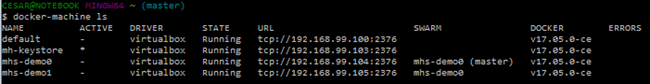
\includegraphics[width=1.2\linewidth]{gfx/master}}\caption[Master node and slaves in Docker]{Master node and slaves in Docker}
{\label{fig:master}
\end{figure}

For the overlay network:
\begin{lstlisting}
$ eval $(docker-machine env --swarm mhs-demo0)
$ docker network create --driver overlay --subnet=10.0.1.0/24 my-network
\end{lstlisting}

Creating the network configuration: \autoref{fig:outside} shows the configuration of the links between docker machines and the created overlay network called my-network for the intercommunication between docker-machines that have inside docker containers.\\

\begin{figure}[bth]
{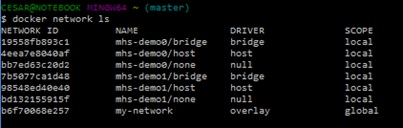
\includegraphics[width=1.1\linewidth]{gfx/outside}}\caption[Network overlay configuration]{Network overlay configuration}
\label{fig:outside}
\end{figure}

In the appendix \autoref{fig:demo0} and \autoref{fig:demo1} shows the configuration of the 2 virtual machines created demo0 and demo1 both hosts are running with the same network id, the same of my-network network, meaning that the multihost network is ready. Next for running an application we need to change the environment to the swarm master and run containers from the master and not from the slaves.\\

This configuration works in the next way: \\

First the mh-keystore is the master node of the configuration, all the instructions that we want to give such as location of the containers within the clusters or the number of replicas that we would like to add for the resilience of the service is given by this master node.\\

The assignment of master and slaves is helpful for the distribution of the data, the master node will have all the information about containers and how do they work, and the slaves will operate and run each particular service.\\


Following the steps of this configuration but implementing OpenvSwitch to the infrastructure to meet the SDN model the service must be isolated.\\

For this it would be very useful to create a container with all the modules and services that are needed to run OpenStack, since containers have all the inter-process communications within the container itself, the computations will be executed inside of the container and it will become a more portable infrastructure.\\

\section{OpenvSwitch configuration for a container deployment}

This part of the project was applied to implement an isolation of the networking component.\\

Because OpenvSwitch is the one that will have all the configuration and information of the location of each container.\\

First in boot2docker which is the virtual environment in which docker is working (we may think of it is as the virtual machine manager), we need to enable the OpenvSwitch kernel module as explained in the architecture of OpenvSwitch in previous sections.\\

Then adding the configuration for the connectivity of the containers as it was shown in the first chapter with the OpenvSwitch.\\

This configuration will be saved after commiting the container, but the configuration of the virtual environment must be previously added manually in every environment.\\
\\

\begin{lstlisting}
modprobe openvswitch
docker run –itd –-cap-add NET_ADMIN socketplane/openvswitch
docker exec <container id ovs> ovs-vsctl add-br s1 
\end{lstlisting}

Note: It is important to notice that I had to do this with my virtual environment since I was using Boot2docker in windows.

\section{Problems and Solutions}

As previously explained in the use of swarm node, the docker toolbox for windows uses swarms to add the docker engine to the nodes.\\

Since the docker engine is the one in charge of the management and storage of information such as process id and state of the containers, in the next chapter because the migration of the containers must be an independent architecture detached from the operating system we need the docker engine to work as a manager for this connections therefore for the next part of the project I will not be able to use the docker toolbox for Windows % Chapter 2
----------------------------------------------------------------------------------------
%	THESIS CONTENT - APPENDICES
%----------------------------------------------------------------------------------------
\let\cleardoublepage\clearpage \appendix
\part{Appendix} % New part of the thesis for the appendix

\let\cleardoublepage\clearpage % Appendix A

\chapter{Appendix}



\section{Appendix}

TTSDASHBOARD interface with data needed to be parsed

\begin{figure}[bth]
{\includegraphics[width=1.2\linewidth]{gfx/ttsdashboard}}\caption[TTS Dashboard interface]{TTS Dashboard interface.}
{\label{fig:ttsdashboard}
\end{figure}

Logfile index seen in kibana: 

\begin{figure}[bth]
{\includegraphics[width=1.1\linewidth]{gfx/logfile}}\caption[Logfile index in kibana]{Logfile index in kibana.}
{\label{fig:Logfile}
\end{figure}

\medskip
\\
\medskip


\clearpage
\\


Rex file format for retreving data:

\begin{figure}[bth]
{\includegraphics[width=1\linewidth]{gfx/logrex}\caption[Rex file format]{Rex file format.}
{\label{fig:logrex}
\end{figure}

Index view in Kibana

\begin{figure}[bth]
{\includegraphics[width=1.2\linewidth]{gfx/index}\caption[Kibana view of indices fields]{Kibana view of indices fields.}
{\label{fig:index}
\end{figure}
\clearpage 

Process of the creation of a new index:
\\
 
\begin{figure}[bth]
{\includegraphics[width=1\linewidth]{gfx/process}\caption[Process of creation of indices]{Process of the creation of new indices.}
{\label{fig:process}
\end{figure}

\clearpage


Data format represented in a tree:

\begin{figure}[bth]
{\includegraphics[width=1\linewidth]{gfx/tree}\caption[Hierarchy of the rex file]{Hierarchy of the rex file.}
{\label{fig:tree}
\end{figure}


\clearpage
\\
	


	
Disk space allocation:

\begin{figure}[bth]
{\includegraphics[width=1\linewidth]{gfx/initial}\caption[Initial allocation]{Inicial allocation.}
{\label{fig:initial}
\end{figure}


Allocation before compression

\begin{figure}[bth]
{\includegraphics[width=1\linewidth]{gfx/without_compression}\caption[Allocation without compression]{Allocation without compression.}
{\label{fig:without_compression}
\vspace{-1.5em}
\end{figure}



Allocation after compression

\begin{figure}[!ht]
\vspace{-1em}
{\includegraphics[width=1\linewidth]{gfx/with_compression}\caption[Allocation with compression]{Allocation with compression.}
{\label{fig:with_compression}
\end{figure}


\begin{figure}[!ht]
\vspace{-1em}
{\includegraphics[width=1\linewidth]{gfx/kibana}\caption[Kibana]{Kibana.}
{\label{fig:kibana}
\end{figure}
 % Appendix A
%% Appendix X

\chapter{Appendix Title}

%----------------------------------------------------------------------------------------

% Content begins here % Appendix B - empty template

%-----------------------------------------------------------------------------

\let\cleardoublepage\clearpage % Bibliography
\chapter{bibliography}
\label{app:bibliography} 
%\begin{thebibliography}{Bibliography}
\bibitem{zen}
[1] IEEE, 2014.
\texit{ Software-Defined Networking: A Comprehensive Survey. Diego Kreutz, Fernando M. V. Ramos, Paulo Verissimo, Christian Esteve Rothenberg, Siamak Azodolmolky, Steve Uhlig}
\\
\bibitem{log}
[2] 2014 Eliza Croen November 1, 2014.
\texit{http://cloudify.co/2014/11/01/openstack-hybrid-cloud-orchestration-TOSCA-NFV-Docker.html}
\\
\bibitem{zen}
[3] Guillaume Urvoy-Keller December 4, 2015	\textit{virtualization-A highlight on performance} 
\\
\bibitem{zen}
[4]
\textit{https://docs.docker.com/get-started/}
\\
\bibitem{zen}
[5]
\textit{https://hub.docker.com/r/anabeldlw/}
\\
\bibitem{log}
[6]
\texit{https://docs.openstack.org/mitaka/networking-guide/deploy-ovs-selfservice.html}
\\
\bibitem{aggs}
[7]
\textit{https://tools.ietf.org/html/rfc7348}
\\
\bibitem{aggs}
[8]
\textit{https://hub.docker.com/r/continuse/openstack-controller/}
\\
\bibitem{aggs}
[9]
\textit{https://docs.openstack.org/mitaka/networking-guide/deploy-ovs-selfservice.html}
\\
\bibitem{aggs}
[10]
\textit{https://docs.openstack.org/ha-guide/intro-ha.html}
\\
\bibitem{log}
[11] Andrey Mirkin, Alexey Kuznetsov, Kolyshkin OpenVZ
\texit{Containers checkpointing and live migration}
\\
\bibitem{log}
[12]
\texit{https://docs.docker.com/engine/installation/linux/docker-ce/ubuntu/#install-using-the-repository}
\\
\bibitem{log}
[13]
\texit{https://download.openvz.org/criu/}
\\
\bibitem{log}
[14]
\texit{http://www.networkcomputing.com/data-centers/docker-containers-9-fundamental-facts/1537300193}
%\end{thebibliography}
 
\end{document}
